\documentclass[journal,compsoc]{IEEEtran}
\usepackage[UKenglish]{babel}
\usepackage[utf8]{inputenc}

\usepackage{graphicx}
\usepackage{mathtools}
\usepackage{amsmath}
\usepackage{url}
\usepackage{listings}
\usepackage{float}
\usepackage{fancyvrb}
\usepackage{framed}
\usepackage{attrib}

\hyphenation{op-tical net-works semi-conduc-tor}

% Styling commands
\newcommand{\tbf}[1]{\textbf{#1}}
\newcommand{\tit}[1]{\textit{#1}}
\newcommand{\ttt}[1]{\texttt{#1}}

% Document-specific commands
\newcommand{\ws}{WebSocket}



\begin{document}

\author{\IEEEauthorblockN{Thibault Gérondal, Michaël Heraly}}

\title{Survey paper: \ws}

\date{Tuesday, 27 Oct 2015}

\maketitle
\IEEEpeerreviewmaketitle


%\IEEEdisplaynontitleabstractindextext

\begin{abstract}
The most common way to get some information and communicate through the internet is via the Hypertext Transfer Protocol (HTTP).
Over time, the shared media sent through this communication system have evolved.
It started from text to images and videos.
And interactions between clients and servers have evolved too.
We went from passive customers who receives informations to active clients that wants to communicate in real-time.
The original HTTP was never designed to achieve those needs.
The market found some tricks to bypass these limitations.
But the HTML5 initiative introduced a real solution to this problem : \ws{}.
This solution brings socket to the web, so a full-duplex communication can be established between the clients and the server.
% This paper is only bullshit, but let's try to sell it.

In this survey paper, we describe the older techniques that were used to achieve a full-duplex communication before describing the \ws{} protocol itself.
Then, we explore some experiments about how \ws{} is efficient compared to these older techniques.
Finally, a point is dedicated to the security issues of \ws.
\end{abstract}


\section{Introduction}

The Hypertext Transfer Protocol (HTTP) is a stateless request-response protocol in the server-client computing model.
The client submits an HTTP request message and the server provides a response (HTML files, images, etc.).
With the growing the popularity of the web, the number of web applications has risen significantly.
And the need of interactivity between the client and the server was increasing.
In the original HTTP specifications, interactivity was only possible by loading an entire page in order to upload informations to the server or to receive new informations from the server.
But new features to web browsers have arisen in order to successfully add interactivity without (re)loading pages.
Among these, two Javascript API were implemented successively in web \mbox{browsers :} XMLHttpRequest and \ws.


\section{XMLHttpRequest}

% Note: real-time interactivity?
One of the first and most used solution to add real-time interactivity is the XMLHttpRequest (XHR) Object which is a Javascript API that permits the browser to send a request for a resource to a distant server.
Despite the name of this API, the fetched resource don't have to be an XML file.
In fact, JSON (JavaScript Object Notation) is generally used as it is more easy to parse in Javascript.
This technique is great to send data to the server but not for receiving new data.
If the client wants to keep the information up to date from the server, it will have to poll the server periodically.
However, doing  that generates a lot of overhead as each request will have a HTTP header and a lot of these requests might return no new data, so this technique is quite ineffective.

\subsection{The long polling version}

The long polling also uses the XMLHttpRequest (XHR) Object.
But, the client doesn't have to poll periodically the server as the web server holds the HTTP request open until it has new data to send to the client, or a timeout expires.
This reduces the amount of useless data transfers and improve the update delay as shown in Fig.~\ref{poll_vs_lpoll}.

\begin{figure}
  \centering
  \label{poll_vs_lpoll}
  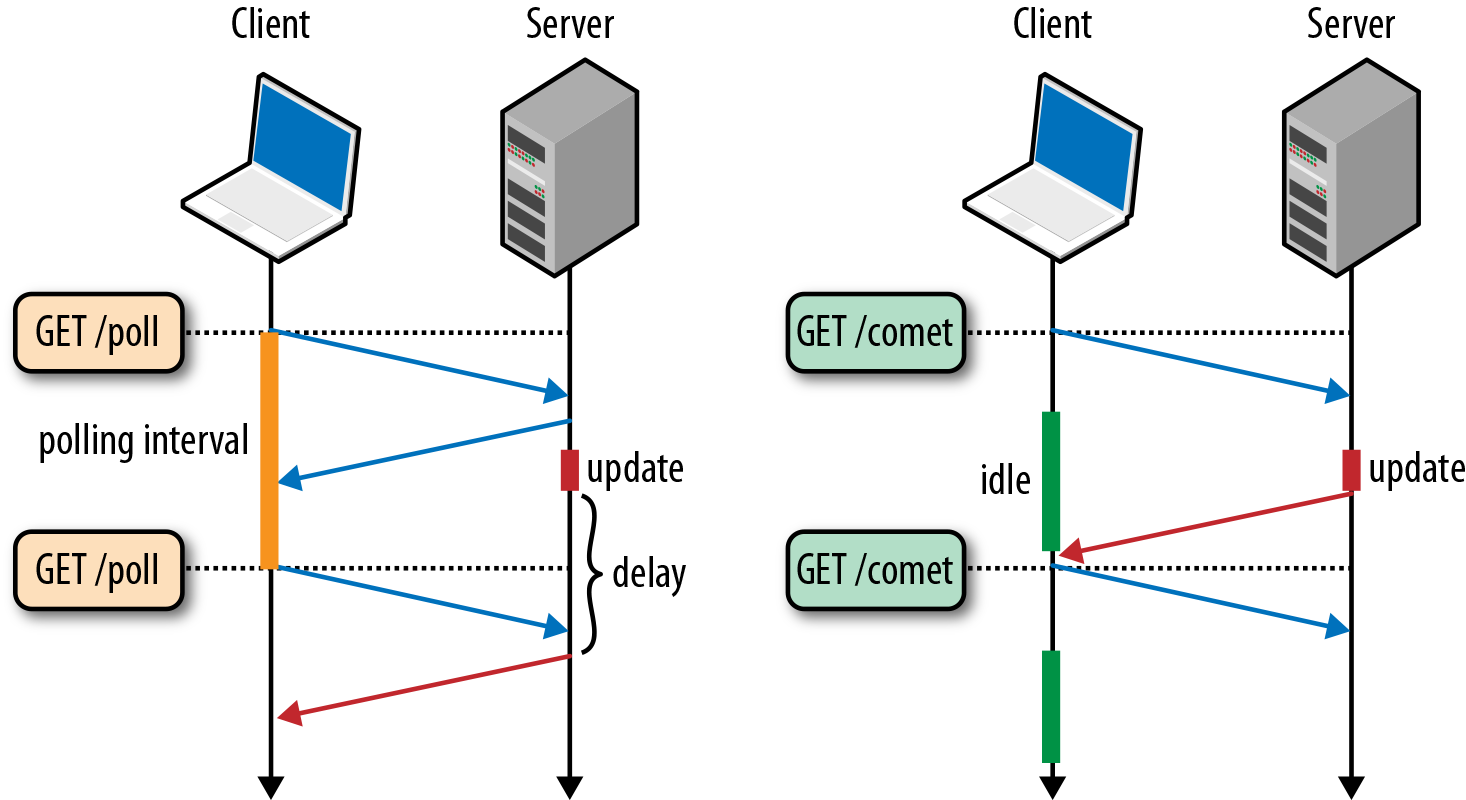
\includegraphics[width=\linewidth]{poll_vs_lpoll}
  \caption{periodic polling (left) versus long polling (right)}
\end{figure}



\section{\ws{} protocol}
The \ws{} protocol was standardized by the IETF as RFC 6455 in 2011 \cite{rfc6455}.
This protocol was designed to bring bidirectional, message-oriented streaming of text and binary data between web browsers and web servers.
As it was designed for the Web, this protocol copes with existing HTTP infrastructure, which means to work over HTTP ports 80 and 443.
But \ws{} remains a fully functional protocol that can be used outside the browser.

\subsection{The \ws{} header}

The \ws{} frame structure is shown in Figure \ref{fig:websocket_frame}.

\begin{figure}
    \centering
    \label{fig:websocket_frame}
    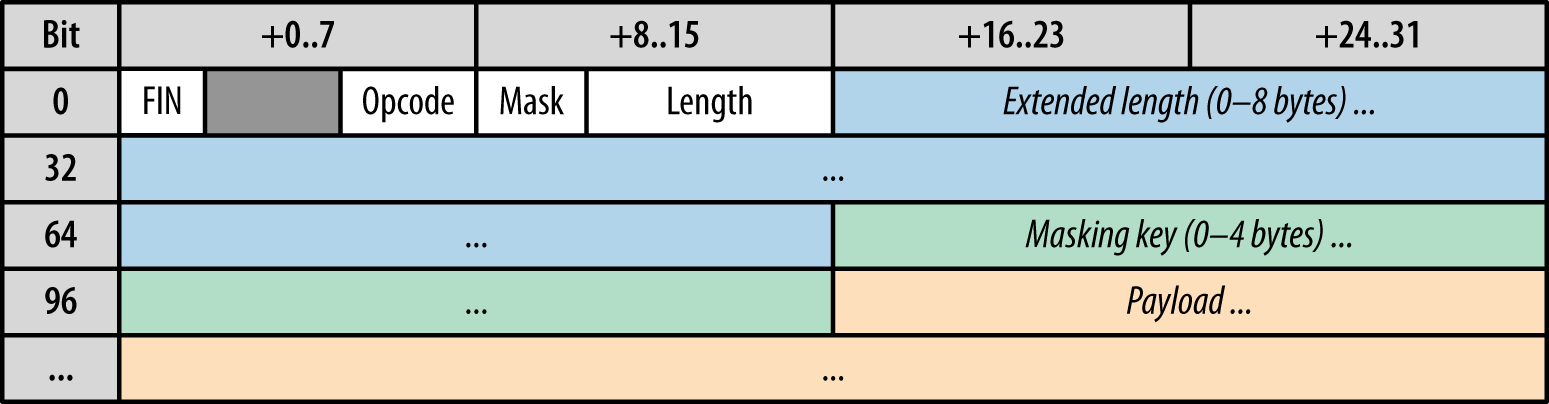
\includegraphics[width=\linewidth]{websocket_frame.png}
    \caption{\ws{} frame structure (from \cite{HighPerfBrowserNetworking:websocket})}
\end{figure}

The \ws{} frame structure is composed of different parts \cite{HighPerfBrowserNetworking:websocket} \cite{performanceEvaluationOfWebsocketProtocol} :
\begin{LaTeXdescription}    % 'description' environment doesn't display well for IEEEtran
    \item[FIN] indicates whether the frame is a final fragment of a message.
    \item[Opcode] indicates the type of the payload data: binary, textual, or protocol-level signaling (e.g. \ttt{close}, \ttt{ping}, \ttt{pong}).
    \item[Mask] indicates whether the payload data is obfuscated (only for messages sent from the client to the server).
    \item[Length] indicates the payload length. If this value is between 0 and 125, this is the actual length.
                    If it is set to 126, the next 2 bytes represent a 16-bit unsigned integer indicating the frame length.
                    If it is set to 127, the next 8 bytes represent a 64-bit unsigned integer indicating the frame length.
    \item[Masking key] used to disable unwanted payload processing by network intermediaries, like HTTP proxies \cite{performanceEvaluationOfWebsocketProtocol}.
                    This part is omitted in server-originated frames, as the masking is not necessary.
    \item[Payload] corresponds to the application data, or custom data if the client and server use a protocol extension.
\end{LaTeXdescription}



\section{\ws{} Javascript API}
The \ws{} Javascript API is being standardized by the World Wide Web Consortium (W3C).


\section{Performance of WebSocket}

Establishing a \ws{} session takes 3.7 times longer than establishing a TCP connection \cite{performanceEvaluationOfWebsocketProtocol}.


\section{\ws{} protocol}

The \ws{} protocol uses the HTTP's \ttt{Upgrade} mechanism as shown in Figure \ref{fig:websocket_connection}.

\begin{figure}
    \centering
    \label{fig:websocket_connection}
    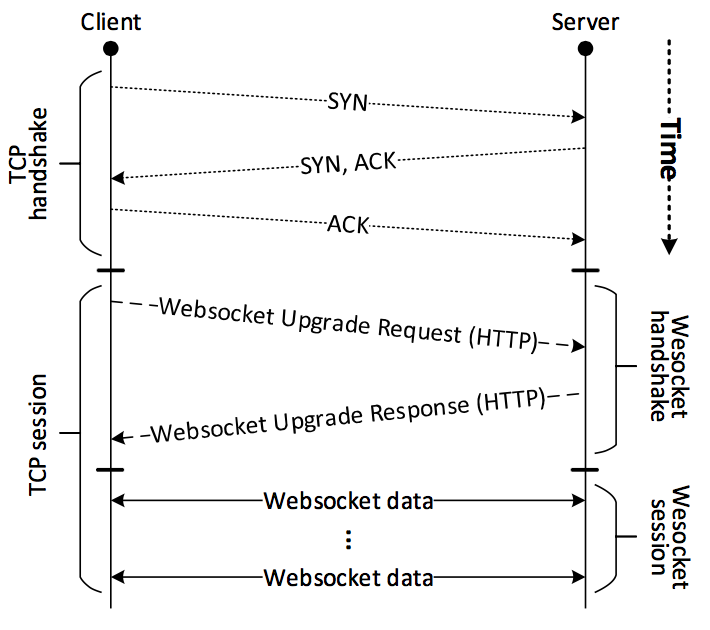
\includegraphics[width=\linewidth]{websocket_tcp_diagram.png}
    \caption{\ws-over-TCP sequence diagram (from \cite{performanceEvaluationOfWebsocketProtocol})}
\end{figure}


\subsection{Presentation}

\subsection{Concrete usage}



\section{Performance of \ws}

\subsection{Comparison with AJAX solutions}

\subsection{Behavior depending on the environment}



\section{Security}

\subsection{CORS}

\subsection{Proxies}



\section{Conclusion}

From a network point of view, \ws …


\ifCLASSOPTIONcaptionsoff
  \newpage
\fi


\bibliographystyle{IEEEtran}
\bibliography{bibi}


\end{document}
